\textbf{COLUNI 2022 -- Questão 25}\par\medskip Leia o texto a seguir.

\par

\textbf{Descoberta abre caminho para antiviral que impeça replicação do Sars-CoV-2}

\par

O RNA do Sars-CoV-2 é protegido por um “envelope” formado por lipídios e proteínas – entre elas, a famosa espícula, que compõe a estrutura de coroa que dá nome à família Coronaviridae. Quando o vírus invade a célula e é englobado por ela, o RNA é liberado da cápsula e as proteínas não estruturais, entre elas a protease principal, entram em cena, atuando no metabolismo viral dentro do hospedeiro. Enquanto as proteínas estruturais costumam servir de alvo para o desenvolvimento de vacinas, as não estruturais são usadas como referência para os medicamentos antivirais. Cientistas desvendaram detalhes do processo de maturação da protease principal em uma investigação realizada no Centro Nacional de Pesquisa em Energia e Materiais (CNPEM), em Campinas, utilizando-se a luz síncrotron. Disponível em: https://cnpem.br/descoberta-abre-caminho-para-antiviral-que-impeca-replicacao-do-sars-cov-2/. Acesso em: 26 ago. 2021. (Adaptado)

% COLUNI-AUTO-FIGURES-BEGIN
\begin{figure}[htbp]
\centering
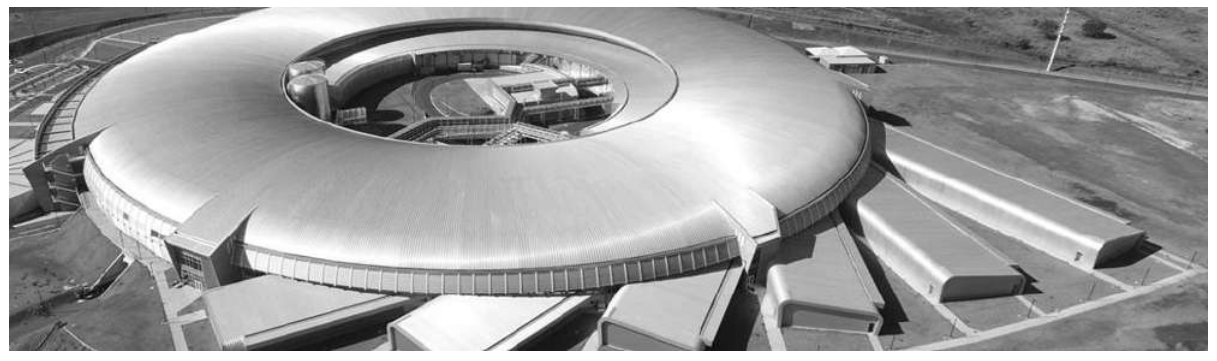
\includegraphics[width=0.95\linewidth]{static/simulados/coluni/figuras/2022/questao-25/figura-1.png}
\end{figure}
% COLUNI-AUTO-FIGURES-END

\par

A luz síncrotron é um tipo de radiação gerada após a aceleração de elétrons. Esses elétrons são mandados para um compartimento tubular circular com vácuo, semelhante ao encontrado no espaço. A trajetória dos elétrons, para seguir essa tubulação circular, é desviada com a ajuda de eletroímãs que atuam nas partículas quando elas estão muito próximas da velocidade da luz. Os elétrons, em alta velocidade, quando desviados da trajetória, acabam gerando a chamada luz síncrotron, que é capaz de atravessar materiais, revelando suas propriedades químicas e estruturais. Esse processo ocorre no Sirius, o acelerador de partículas brasileiro. Disponível em: https://cnpem.br/. Acesso em: 03 set. 2021. (Adaptado)

\par

Com base nas informações fornecidas e nos conhecimentos sobre ciências, assinale a afirmativa CORRETA:


\begin{enumerate}
\item Os prótons poderiam ser utilizados no lugar dos elétrons, na produção de luz síncrotron, pois ambas as
       partículas apresentam o mesmo valor de massa.
\item A aceleração de elétrons só é possível tendo em vista o fato deles serem partículas neutras e estarem
       localizados na eletrosfera dos átomos.
\item Os elétrons precisam ser acelerados para adquirir energia suficiente e abandonar o interior dos núcleos
       dos átomos dos quais eles fazem parte.
\item Os átomos, ao perderem os elétrons que serão utilizados no acelerador de partículas, originam estruturas
       positivas chamadas de cátions.\end{enumerate}
